\documentclass{beamer}
%
% Choose how your presentation looks.
%
% For more themes, color themes and font themes, see:
% http://deic.uab.es/~iblanes/beamer_gallery/index_by_theme.html
%
\mode<presentation>
{
  \usetheme{default}      % or try Darmstadt, Madrid, Warsaw, ...
  \usecolortheme{default} % or try albatross, beaver, crane, ...
  \usefonttheme{default}  % or try serif, structurebold, ...
  \setbeamertemplate{navigation symbols}{}
  \setbeamertemplate{caption}[numbered]
} 

\usepackage[english]{babel}
\usepackage[utf8]{inputenc}
\usepackage[T1]{fontenc}
\usepackage{amsmath, amssymb}
\usepackage{subcaption}
\usepackage{textcomp}
\usepackage{array,multirow,graphicx}
\usepackage{booktabs}

\title[Assignment 1]{Information Retrieval Assignment 1\\Vector-Space Model}
\author{Andrew McIsaac}
\date{December 7, 2021}

\begin{document}

\begin{frame}
  \titlepage
\end{frame}

\section{Preprocessing}

\begin{frame}{Index Construction}

\begin{itemize}
  \item Czech tags: [Geography, Title, Heading, Text]
  \item English tags: [PH, KH, HD, DH, SE, DL, LD, TE, CP, DC, CR, DP, SM]
  \item Inverted Index
	  \begin{itemize}
		\item (docID, term) pairs for every document and every term
		\item Invert with SPIMI-Index
	  	\item Sorted terms and postings list for documents of every file
		\item Merge to final inverted index and write to disk
	  \end{itemize}
\end{itemize}

\end{frame}

\section{Baseline Results}

\begin{frame}{Baseline Results}

\begin{itemize}
	\item Czech: 0.0597 MAP, 0.084 $P_{10}$
	\item English: 0.0445 MAP, 0.084 $P_{10}$
\end{itemize}

\end{frame}

\section{Experiments}

\begin{frame}{Preprocessing}
\begin{itemize}
  \item Lemmas - \texttt{spacy}, \texttt{spacy\_udpipe}
  \item Stemming - Porter Stemmer
  \item Stopwords - from \texttt{spacy}
\end{itemize}

\begin{table}[htpb]
	\centering
	\caption{Mean average precision (MAP) and $P_{10}$ precision of the first 10
		documents training performance with different preprocessing techniques.\\
	wf: word forms, sw: stopwords, l: lemmatization, s: stemming\\}
	\label{tab:terms}
	\begin{tabular}{@{}l|ccccc@{}}
		\toprule
		Language & & wf & sw & sw+l & sw+s \\
		\cmidrule(r){1-1}\cmidrule(lr){2-2}\cmidrule(lr){3-3}\cmidrule(lr){4-4}\cmidrule(lr){5-5}\cmidrule(l){6-6}
		English & MAP & 0.0445 & 0.1244 & 0.0834 & \textbf{0.1751} \\
				& \small{$P_{10}$} & \small{0.084} & \small{0.172} & \small{0.136} & \small{0.252} \\
		\cmidrule(r){1-1}\cmidrule(lr){2-2}\cmidrule(lr){3-3}\cmidrule(lr){4-4}\cmidrule(lr){5-5}\cmidrule(l){6-6}
		Czech & MAP & 0.0597 & 0.0770 & \textbf{0.1553} & 0.0672 \\
			  & \small{$P_{10}$} & \small{0.084} & \small{0.100} & \small{0.148} & \small{0.060} \\
		\bottomrule
	\end{tabular}
\end{table}

\end{frame}

\subsection{Term/Document Frequency Weighting}

\begin{frame}{Term/Document Frequency Weighting}

\begin{table}[htpb]
	\centering
	\caption{Mean average precision (MAP) and $P_{10}$ precision of the first
		10 documents training performance with different tf-idf weightings.\\
	SMART notation tags are applied to both query and document in all cases.\\}
	\label{tab:tfidf}
	\begin{tabular}{@{}l|cccccc@{}}
		\toprule
		Language & & nnc & ntc & npc & ltc & apc \\
		\cmidrule(r){1-1}\cmidrule(lr){2-2}\cmidrule(lr){3-3}\cmidrule(lr){4-4}\cmidrule(lr){5-5}\cmidrule(lr){6-6}\cmidrule(l){7-7}
		English & MAP & 0.1751 & 0.2244 & \textbf{0.2248} & 0.1320 & 0.0469 \\
				& \small{$P_{10}$} & \small{0.252} & \small{0.328} & \small{0.328} & \small{0.172} & \small{0.092} \\
		\cmidrule(r){1-1}\cmidrule(lr){2-2}\cmidrule(lr){3-3}\cmidrule(lr){4-4}\cmidrule(lr){5-5}\cmidrule(lr){6-6}\cmidrule(l){7-7}
		Czech & MAP & 0.1553 & 0.1933 & \textbf{0.1947} & 0.0879 & 0.0922 \\
		& \small{$P_{10}$} & \small{0.148} & \small{0.224} & \small{0.228} & \small{0.096} & \small{0.100} \\
		\bottomrule
	\end{tabular}
\end{table}

\end{frame}

\subsection{Pivoted Document Length Normalization}

\begin{frame}{Pivoted Document Length Normalization}

\begin{figure}[htpb]
	\centering
	\begin{subfigure}{0.45\textwidth}
		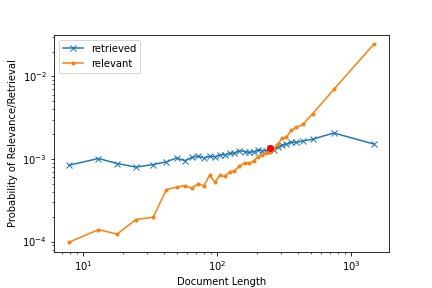
\includegraphics[width=\textwidth]{plot_cs_rel_ret.jpg}
		\caption{Czech}
		\label{fig:cs_cosine}
	\end{subfigure}
	\hfill
	\begin{subfigure}{0.45\textwidth}
		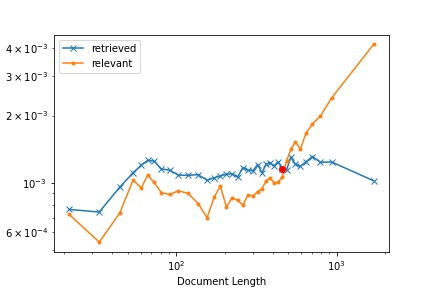
\includegraphics[width=\textwidth]{plot_en_rel_ret.jpg}
		\caption{English}
		\label{fig:en_cosine}
	\end{subfigure}
	\caption{Document lengths for retrieval using cosine normalization compared
	to relevance.}
	\label{fig:cosine}
\end{figure}

\end{frame}

\begin{frame}{Pivoted Document Length Normalization}

\begin{table}[htpb]
	\centering
	\caption{MAP training performance of pivoted document length normalization 
	with different values of scaling factor $a$\\}
	\label{tab:pivot}
	\begin{tabular}{@{}lccccccc@{}}
		\toprule
		& 0.6 & 0.7 & 0.8 & 0.85 & 0.9 & cosine \\
		\cmidrule(r){1-1}\cmidrule(lr){2-2}\cmidrule(lr){3-3}\cmidrule(lr){4-4}\cmidrule(lr){5-5}\cmidrule(lr){6-6}\cmidrule(l){7-7}
		English & 0.2428 & 0.2442 & 0.2446 & \textbf{0.2453} & 0.2450 & 0.2248 \\
		\cmidrule(r){1-1}\cmidrule(lr){2-2}\cmidrule(lr){3-3}\cmidrule(lr){4-4}\cmidrule(lr){5-5}\cmidrule(lr){6-6}\cmidrule(l){7-7}
		Czech & 0.1830 & 0.1869 & 0.1932 & 0.1938 & \textbf{0.2053} & 0.1947 \\
		\bottomrule
	\end{tabular}
\end{table}

\end{frame}

\begin{frame}{Pivoted Document Length Normalization}

\begin{figure}[htpb]
	\centering
	\begin{subfigure}{0.3\textwidth}
		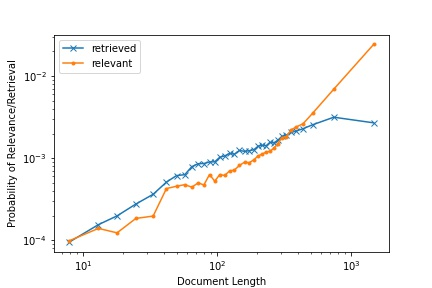
\includegraphics[width=\textwidth]{plot_cs_rel_ret_pivoted0_6.jpg}
		\caption{Czech, $a = 0.6$}
		\label{fig:cs_pivot}
	\end{subfigure}
	\hfill
	\begin{subfigure}{0.3\textwidth}
		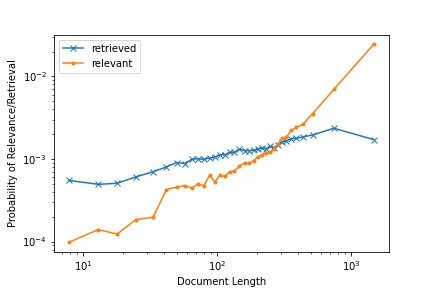
\includegraphics[width=\textwidth]{plot_cs_rel_ret_pivoted0_9.jpg}
		\caption{Czech, $a = 0.9$}
		\label{fig:cs_pivot}
	\end{subfigure}
	\hfill
	\begin{subfigure}{0.3\textwidth}
		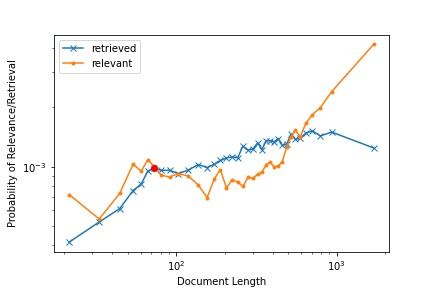
\includegraphics[width=\textwidth]{plot_en_rel_ret_pivoted.jpg}
		\caption{English, $a = 0.85$}
		\label{fig:en_pivot}
	\end{subfigure}
	\caption{Document lengths for retrieval using pivoted document length
	normalization compared to relevance.}
	\label{fig:pivot}
\end{figure}

\end{frame}

\section{Problems}

\begin{frame}{Problems}

\begin{itemize}

	\item<1-> Not enough RAM so index construction would crash
		\begin{itemize}
			\item<2-> Close Firefox, Spotify
		\end{itemize}
	\item<3-> Queries took a very long time (>20 minutes)
	\begin{itemize}
		\item<4-> Use \texttt{pd.DataFrame} to index by doc name instead
		\item<4-> Now much quicker
	\end{itemize}
	\item<5-> \texttt{nltk} has no Czech stemmer
		\begin{itemize}
			\item<6-> Find it online
			\item<6-> But maybe it wasn't very good\ldots
		\end{itemize}
	\item<7-> \texttt{spacy} has no Czech lemmatizer
		\begin{itemize}
			\item<8-> Use \texttt{spacy\_udpipe}
			\item<8-> But it was much slower\ldots
		\end{itemize}

\end{itemize}

\end{frame}

\end{document}
